\input ../preamble

\begin{document}

{\Huge

  \centerline{\bf TTIC 31230, Fundamentals of Deep Learning}
  \bigskip
  \centerline{David McAllester, Winter 2018}

    \vfill
  \centerline{\bf Convolutional Neural Networks --- CNNs}
\ignore{
  \vfill
  \centerline{\bf Review of EDF and Explicit Index Notation}
  \vfill
  \centerline{\bf Convolutional Neural Networks --- CNNs}
  \vfill
  \centerline{\bf Initialization and Batch Normalization}
  \vfill
  \centerline{\bf Skip Connections (Resnet)}
}
  \vfill
  \vfill


\slide{CNNs}

Imagenet Classification. 1000 kinds of objects.

\vfill
\centerline{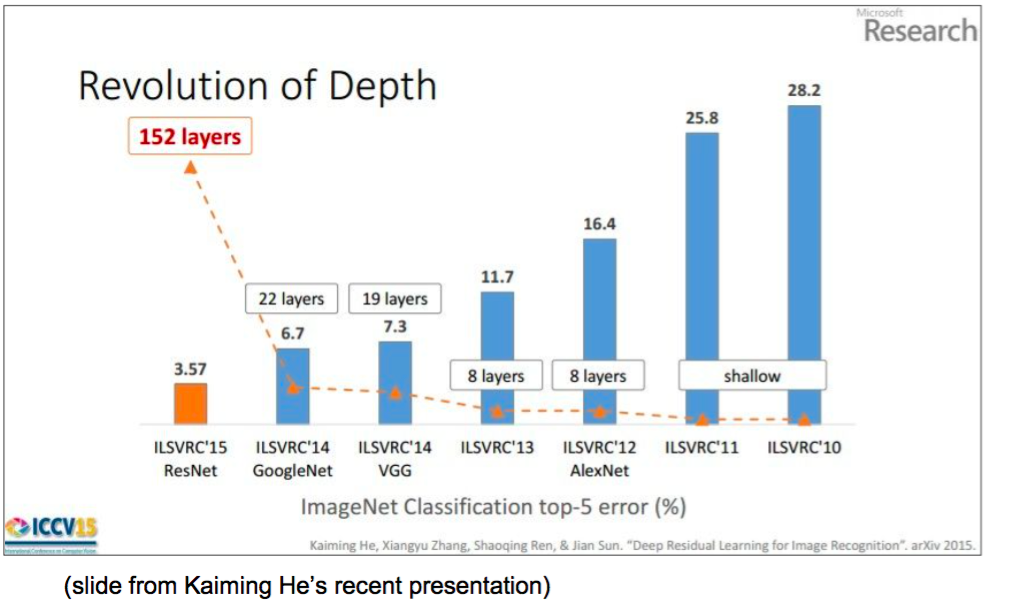
\includegraphics[height=4.5in]{../images/IVLSRC}}
2016 error rate is 3.0\% \hspace{1.0in} 2017 error rate is 2.25\%


\slideplain{A CNN}

A convolution slides a filter (a kernel) across an image.

\centerline{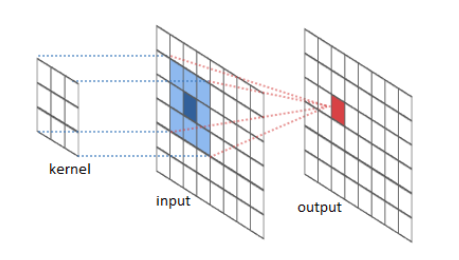
\includegraphics[width = 3.5in]{../images/Convolution}}
\centerline{$W$\hspace{6ex}$x$\hspace{6ex}$y$}
\centerline{\large River Trail Documentation}

\begin{eqnarray*}
  y[b,i,j,c_y] & = &   W[\Delta i, \Delta j, c_x, c_y] x[b,i + \Delta i, j + \Delta j, c_x] \\
  \\
  y[b,i,j,c_y] & \pluseq & B[c_y]
  %W.\mathrm{grad}[\Delta i, \Delta j,c_x,c_y] & \pluseq & y.\mathrm{grad}[b,i,j,c_y]x[b,i + \Delta i,j+ \Delta_j,c_x]
\end{eqnarray*}

\slide{Use Swap Rule to get Backward Method}

\begin{eqnarray*}
  y[b,i,j,c_y] & = &   W[\Delta i, \Delta j, c_x, c_y] x[b,i + \Delta i, j + \Delta j, c_x] \\
  \\
  W.\mathrm{grad}[\Delta i, \Delta j,c_x,c_y] & \pluseq & y.\mathrm{grad}[b,i,j,c_y]x[b,i + \Delta i,j+ \Delta_j,c_x]
\end{eqnarray*}

$$x.\mathrm{grad}[b,i+\Delta i,j+\Delta j,c_x] \;\pluseq \; W[\Delta i, \Delta j, c_x, c_y] y.\mathrm{grad}[b,i,j,c_y]$$

\slide{A Convolution Class in EDF}

In EDF we would define a class for convolution parameter packages.

\vfill
We would then construct the computation node for the output using Python code.

\vfill
\centerline{\tt Y = Relu(Conv(Phi,X)).}

\slide{Padding}

\centerline{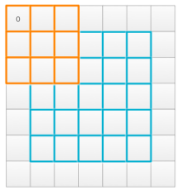
\includegraphics[height = 2.0in]{../images/padding2}}
\centerline{\large Jonathan Hui}

\vfill
If we pad the input with zeros then the input and output can have the same spatial dimensions.

\slide{Zero Padding in NumPy}

In NumPy we can add a zero padding of width p to an image as follows:

\vfill
\begin{verbatim}
padded = np.zeros(W + 2*p,  H + 2*p)

padded[p:W+p, p:H+p] = x
\end{verbatim}

\slide{Padding}

\centerline{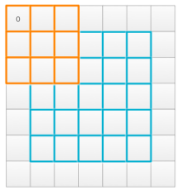
\includegraphics[height = 2.0in]{../images/padding2}}
\centerline{\large Jonathan Hui}

Let $x'$ (full square) be the padding of $x$ (blue square).  $y$ also has the blue shape.

\vfill
$$y[b,i,j,c_y]  =   W[\Delta i, \Delta j, c_x, c_y] x'[b,i + \Delta i, j + \Delta j, c_x] + B[c_y]$$

\vfill
\vfill
For padding $p$ and a filter of width $2p+1$, we get that $y$ has the same spatial dimensions as $x$.


\slide{Strides}

We can move the filter by a ``stride'' $s$ for each spatial step.

\vfill
\begin{eqnarray*}
  y[b,i,j,c_y] & = &  W[\Delta i, \Delta j, c_x, c_y] x[b,s*i + \Delta i, s*j + \Delta j, c_x] + B[c_y]
\end{eqnarray*}

\slide{Max Pooling}

$$y[b,i,j,c] = \max_{\Delta i, \Delta j}\; x[b,s*i + \Delta i,\; s*j + \Delta j,\; c]$$

\vfill
This is typically done with a stride greater than one so that the image dimension is reduced.



\slide{Fully Connected (FC) Layers}

We reshape $x[b,x,y,c]$ to $x[b,(x,y,c)]$ and convert to using an MLP.

\slide{Basics}

\begin{itemize}
\item Padding

  \vfill
\item Convolution

  \vfill
\item Stides

  \vfill
\item Max Pooling

  \vfill
\item Fully Connected Layers
\end{itemize}

\slide{A Sequence of ``Images''}

\centerline{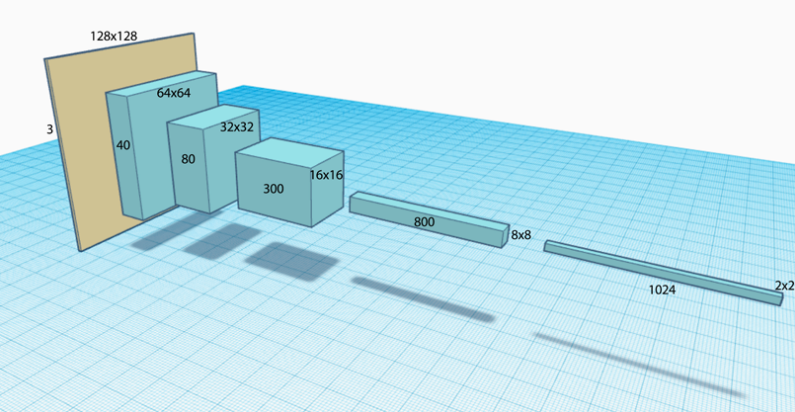
\includegraphics[width= 8.5in]{../images/Stack}}
\centerline{\large Jonathan Hui}

\slide{Alexnet}
\centerline{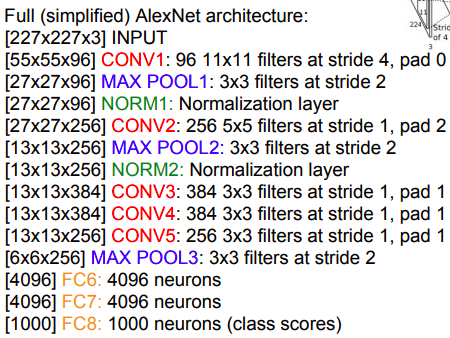
\includegraphics[height=4.5in]{../images/AlexnetStack}}
\centerline{\large Stanford CS231}

\slide{VGG, Zisserman, 2014}

\centerline{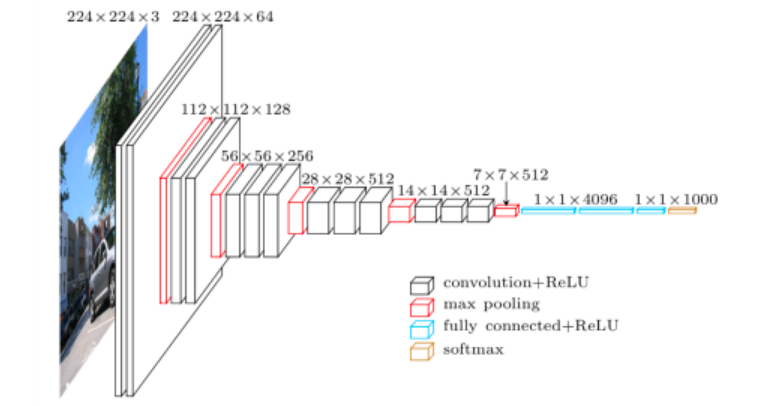
\includegraphics[width = 9.0in]{../images/VGG}}
\centerline{\large Davi Frossard}

\slide{VGG}
\centerline{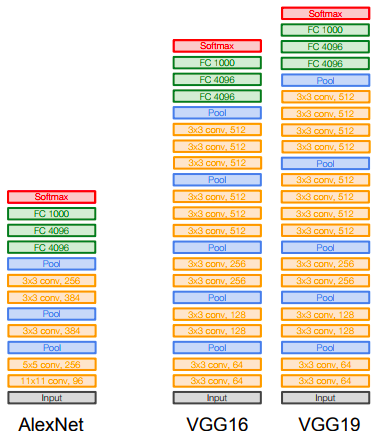
\includegraphics[height=4.5in]{../images/VGGStack}}
\centerline{\large Stanford CS231}

\slide{Inception, Google, 2014}

\centerline{\includegraphics[width = 9.0in]{../images/inception1}}
\vfill
\centerline{\includegraphics[width = 3.5in]{../images/inception2}}

\slide{Imagenet Classification}

1000 kinds of objects.

\vfill
\centerline{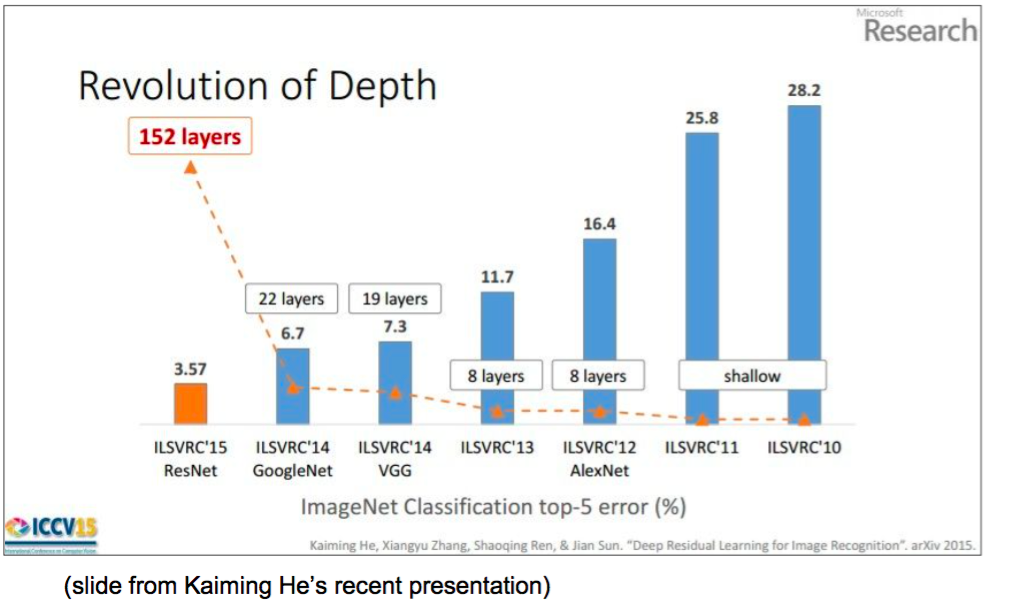
\includegraphics[height=4.5in]{../images/IVLSRC}}
2016 error rate is 3.0\% \hspace{1.0in} 2017 error rate is 2.25\%

\slideplain{Appendix: Image to Column (Im2C)}

Reduce convolution to matrix multiplication ---  more space but faster.
{\huge
  $$x'[b,i,j,\Delta i,\Delta j,c_x] = x[b,i+\Delta i,j+\Delta j,c_x]$$

\begin{eqnarray*}
  & & y[b,i,j,c_y] \\
  \\
  & = & \left(\sum_{\Delta i, \Delta j, c_x} W[\Delta i, \Delta j, c_x, c_y] *x[b,i + \Delta i,\; j + \Delta j,\; c_x]\right) + B[c_y] \\
  \\
      & = & \left(\sum_{\Delta i, \Delta j, c_x} \begin{array}{l}
                                              x'[b,i,j,\Delta i,\Delta j,c_x]
                                              * W[\Delta i, \Delta j, c_x, c_y] \\
  \end{array}\right) + B[c_y] \\
  \\
    & = & \left(\sum_{(\Delta i, \Delta j, c_x)} \begin{array}{l}
                                              x'[(b,i,j),(\Delta i,\Delta j,c_x)]
                                              * W[(\Delta i, \Delta j, c_x), c_y] \\
                                           \end{array}\right) + B[c_y]
\end{eqnarray*}
}

\slideplain{Appendix: Dilation}

We can ``dilate'' the filter by introducing an image step size $d$ for each step in the filter coordinates.

\vfill
\begin{eqnarray*}
  y[b,i,j,c_y] & = &  W[\Delta i, \Delta j, c_x, c_y] x[b,i + d*\Delta i, j + d*\Delta j, c_x] + B[c_y]
\end{eqnarray*}




\slideplain{END}

}
\end{document}
